\documentclass{beamer}
\usepackage[utf8]{inputenc}
\usepackage{listings}
\usepackage{color}
\usetheme{Madrid}
\title[Bindings]{Bindings}
\author{Rafael Fernández López}
\institute{Artesanos}
\date{}

\pdfinfo
{
  /Title       (BINDINGS)
  /Author      (RAFAEL FERNANDEZ LOPEZ)
}

\definecolor{gray97}{gray}{.97}
\definecolor{gray75}{gray}{.75}
\definecolor{gray45}{gray}{.45}

\lstset{ frame=Ltb,
         framerule=0pt,
         aboveskip=0.5cm,
         framextopmargin=3pt,
         framexbottommargin=3pt,
         framexleftmargin=0.4cm,
         framesep=0pt,
         rulesep=.4pt,
         backgroundcolor=\color{gray97},
         rulesepcolor=\color{black},
         %
         stringstyle=\ttfamily,
         showstringspaces = false,
         basicstyle=\scriptsize\ttfamily,
         commentstyle=\color{gray45},
         keywordstyle=\bfseries,
         %
         numbers=left,
         numbersep=-5pt,
         numberstyle=\tiny,
         numberfirstline = false,
         breaklines=true
      }

\setbeamertemplate{navigation symbols}{}

\begin{document}

\begin{frame}
  \titlepage
\end{frame}

\section*{}
\begin{frame}{}
  \framesubtitle{}
  \tableofcontents[section=1]
\end{frame}

\newcommand<>{\highlighton}[1]{%
  \alt#2{\structure{#1}}{{#1}}
}

\newcommand{\icon}[1]{\pgfimage[height=1em]{#1}}

\section{Definición}

\begin{frame}{¿Qué es un Binding?}
  \begin{itemize}
    \item Un Binding es la creación de una sencilla referencia a algo que es más grande, más complicado y
          más frecuentemente utilizado
    \smallskip
    \begin{figure}[H]
        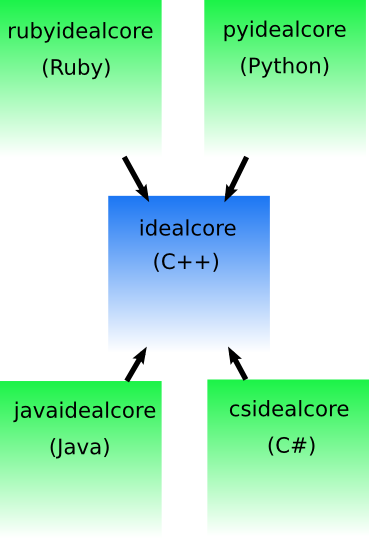
\includegraphics[scale=0.2]{idealbindings.png}
    \end{figure}
  \end{itemize}
\end{frame}

\begin{frame}{¿Por qué escribir Bindings?}
  \begin{itemize}
    \item Amplían potencialmente el número de personas interesadas en la tecnología
    \medskip
    \item Ayudan a encontrar:
    \begin{itemize}
      \item Bugs en la librería
      \item Fallos de diseño
    \end{itemize}
  \end{itemize}
\end{frame}

\section{Cómo escribirlos}

\begin{frame}{Un Binding convencional (C)}
   \framesubtitle{Python}
   \begin{itemize}
     \item Escrito en C
     \medskip
     \item Exporta símbolos al lenguaje destino (Python en este caso)
     \medskip
     \item Puente para realizar y recibir llamadas. El código ejecutado es el código objeto original (C compilado en este caso, ensamblador)
     \medskip
     \item Costoso para el creador del Binding
     \begin{itemize}
       \item Pequeños cambios en la API original pueden provocar una completa reescritura del Binding
     \end{itemize}
     \medskip
     \item Cambios en la propia arquitectura del lenguaje para la creación de Bindings
   \end{itemize}
\end{frame}

\frame{
  \frametitle{}
  \vspace{1.5cm}
  {\huge \textbf{Unos ejemplos...}}
}

\section{SWIG}

\begin{frame}{¿Qué es SWIG?}
  \begin{itemize}
    \item SWIG es un compilador de interfaces que conecta programas escritos en C y C++ con lenguajes como:
    \begin{itemize}
        \item Perl
        \item Python
        \item Ruby
        \item Tcl
    \end{itemize}
    \medskip
    \item Funciona recogiendo las declaraciones encontradas en:
    \begin{itemize}
      \item El fichero de interfaz de SWIG
      \item Las cabeceras C/C++
    \end{itemize}
  \end{itemize}
\end{frame}

\frame{
  \frametitle{}
  \vspace{1.5cm}
  {\huge \textbf{Unos ejemplos...}}
}

\frame{
  \frametitle{}
  \vspace{1.5cm}
  {\huge \alert{\textbf{Gracias.}} ¿Preguntas?}

  \vspace{3.5cm}
  \begin{flushright}
    Rafael Fernández López

    \structure{\footnotesize{ereslibre@kde.org}}
  \end{flushright}
}

\end{document}
